\documentclass{article}
\usepackage{arxiv}

\usepackage[utf8]{inputenc}
\usepackage[english, russian]{babel}
\usepackage[T1]{fontenc}
\usepackage{url}
\usepackage{booktabs}
\usepackage{amsfonts}
\usepackage{nicefrac}
\usepackage{microtype}
\usepackage{lipsum}
\usepackage{graphicx}
\usepackage{natbib}
\usepackage{doi}



\title{	Классические методы как регуляризатор при генерации диффузионных моделей }

\author{ Войт Руслан Александрович \\
	факультет ВМК\\
	МГУ им. М.В. Ломоносова\\
	Москва \\
}
\date{2025}

\renewcommand{\shorttitle}{\textit{arXiv} Template}

%%% Add PDF metadata to help others organize their library
%%% Once the PDF is generated, you can check the metadata with
%%% $ pdfinfo template.pdf
\hypersetup{
pdftitle={	Классические методы как регуляризатор при генерации диффузионных моделей },
pdfsubject={q-bio.NC, q-bio.QM},
pdfauthor={Войт Руслан Александрович},
pdfkeywords={диффузионные модели, регуляризация, структурные дескрипторы, медиальная ось, диаграмма Вороного},
}

\begin{document}
\maketitle

\begin{abstract}
	В работе исследуется применение классических методов компьютерного зрения для регуляризации процесса генерации в диффузионных моделях. Предлагается использовать структурные дескрипторы, такие как диаграмма Вороного, медиальная ось и контурный анализ, для наложения ограничений на процесс денойзинга. Это позволяет генерировать изображения с улучшенной структурной целостностью, топологической точностью и четкими границами объектов. Эксперименты показывают, что предложенный подход эффективно подавляет артефакты генерации и повышает семантическую согласованность выходных данных, особенно в задачах, требующих точного воспроизведения геометрии сцены.
\end{abstract}


\keywords{Диффузионные модели \and Регуляризация \and Медиальная ось \and Диаграмма Вороного}

\section{Introduction}

Современные диффузионные модели демонстрируют выдающиеся результаты в генерации изображений, однако сталкиваются с проблемами структурной целостности и топологической точности генерируемых данных. Такие артефакты, как нарушение геометрии объектов, разрывы контуров и семантическая несогласованность, ограничивают применение этих моделей в задачах, требующих точного воспроизведения структуры сцены. Необходимость регуляризации генеративного процесса становится особенно актуальной в контексте проблемы запоминания обучающих данных и нарушения нормальности обратного процесса~\cite{baptista2025memorizationregularizationgenerativediffusion, falck2025fourierspaceperspectivediffusion}.

Существующие подходы к регуляризации диффузионных моделей включают различные методы структурной стилизации. В работах~\cite{chen2024contourdiffunpairedimagetoimagetranslation, pobitzer2024outlineguidedobjectinpaintingdiffusion} предлагается использование контурных представлений для сохранения анатомической структуры при междоменном переводе изображений. Методы скелетной стилизации ~\cite{ju2023humansdnativeskeletonguideddiffusion, zhu2023diffusionmodeleventskeleton} демонстрируют эффективность структурного контроля при генерации сложных объектов. Перспективным направлением является использование топологических инвариантов, как в работе~\cite{gupta2024topodiffusionnet}, где персистентная гомология используется для контроля чисел Бетти. Классические методы компьютерного зрения, такие как морфологическая диффузия~\cite{angulo2011generalisedmorphologicalimagediffusion} и анизотропная регуляризация~\cite{Pace2013-da}, также находят применение в современных генеративных моделях.

Несмотря на разнообразие существующих подходов, большинство методов не обеспечивают комплексного учета структурных характеристик различного уровня. Использование отдельных дескрипторов (контуры, скелеты) ограничивает возможность контроля глобальной топологии сцены. Кроме того, многие решения требуют значительной модификации архитектуры модели или сложных процедур обучения, что снижает их практическую применимость. Частотный анализ~\cite{falck2025fourierspaceperspectivediffusion} показывает, что стандартные процессы диффузии неравномерно зашумляют различные частотные компоненты, что приводит к потере структурных деталей.

В данной работе предлагается унифицированный подход к регуляризации диффузионных моделей на основе классических структурных дескрипторов компьютерного зрения. Мы используем диаграммы Вороного, медиальные оси и контурный анализ для создания многоуровневых ограничений на процесс денойзинга. Предлагаемый метод позволяет непосредственно встраивать структурные априорные предположения в генеративный процесс без существенного изменения архитектуры модели. Для интеграции классических дескрипторов разработаны специализированные функции потерь и механизмы внимания, обеспечивающие согласованность на различных уровнях абстракции.

Экспериментальные результаты демонстрируют, что предложенный подход значительно улучшает структурную целостность и топологическую точность генерируемых изображений по сравнению с современными методами. Был разработан унифицированный фреймворк для интеграции классических методов компьютерного зрения в современные диффузионные модели, что открывает новые возможности для точного контроля геометрии генерируемых сцен. Предложенное решение эффективно подавляет артефакты генерации и повышает семантическую согласованность, особенно в задачах, требующих точного воспроизведения сложных структур.

\section{Headings: first level}
\label{sec:headings}

\lipsum[4] See Section \ref{sec:headings}.

\subsection{Headings: second level}
\lipsum[5]
\begin{equation}
	\xi _{ij}(t)=P(x_{t}=i,x_{t+1}=j|y,v,w;\theta)= {\frac {\alpha _{i}(t)a^{w_t}_{ij}\beta _{j}(t+1)b^{v_{t+1}}_{j}(y_{t+1})}{\sum _{i=1}^{N} \sum _{j=1}^{N} \alpha _{i}(t)a^{w_t}_{ij}\beta _{j}(t+1)b^{v_{t+1}}_{j}(y_{t+1})}}
\end{equation}

\subsubsection{Headings: third level}
\lipsum[6]

\paragraph{Paragraph}
\lipsum[7]



\section{Examples of citations, figures, tables, references}
\label{sec:others}

\subsection{Citations}
Citations use \verb+natbib+. The documentation may be found at
\begin{center}
	\url{http://mirrors.ctan.org/macros/latex/contrib/natbib/natnotes.pdf}
\end{center}

Here is an example usage of the two main commands (\verb+citet+ and \verb+citep+): Some people thought a thing \citep{kour2014real, hadash2018estimate} but other people thought something else \citep{kour2014fast}. Many people have speculated that if we knew exactly why \citet{kour2014fast} thought this\dots

\subsection{Figures}
\lipsum[10]
See Figure \ref{fig:fig1}. Here is how you add footnotes. \footnote{Sample of the first footnote.}
\lipsum[11]

\begin{figure}
	\centering
	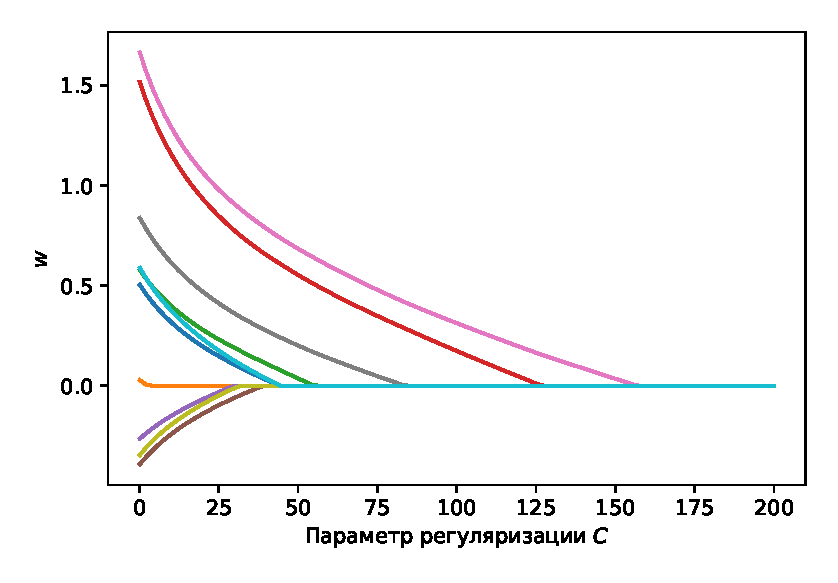
\includegraphics[width=0.5\textwidth]{../figures/log_reg_cs_exp.eps}
	\caption{Sample figure caption.}
	\label{fig:fig1}
\end{figure}

\subsection{Tables}
See awesome Table~\ref{tab:table}.

The documentation for \verb+booktabs+ (`Publication quality tables in LaTeX') is available from:
\begin{center}
	\url{https://www.ctan.org/pkg/booktabs}
\end{center}


\begin{table}
	\caption{Sample table title}
	\centering
	\begin{tabular}{lll}
		\toprule
		\multicolumn{2}{c}{Part}                   \\
		\cmidrule(r){1-2}
		Name     & Description     & Size ($\mu$m) \\
		\midrule
		Dendrite & Input terminal  & $\sim$100     \\
		Axon     & Output terminal & $\sim$10      \\
		Soma     & Cell body       & up to $10^6$  \\
		\bottomrule
	\end{tabular}
	\label{tab:table}
\end{table}

\subsection{Lists}
\begin{itemize}
	\item Lorem ipsum dolor sit amet
	\item consectetur adipiscing elit.
	\item Aliquam dignissim blandit est, in dictum tortor gravida eget. In ac rutrum magna.
\end{itemize}


\bibliographystyle{unsrtnat}
\bibliography{references}

\end{document}